\section{Theorie}
\label{sec:theorie}

%In diesem Abschnitt wird das Prinzip der Interferenz erläutert, welches die Grundlage für das Michelson-Interferometer bildet.

Licht breitet sich im einfachsten Fall als ebene Welle der Form 
\begin{equation}
    \vec{E}(x,t) = \vec{E_0} \cos(kx - \omega t + \delta)
    \label{eq:ebenewellen}
\end{equation}
aus, dabei ist k die Wellenzahl, $\omega$ die Kreisfrequenz und $\delta$ der Phasenwinkel. \\

Für Licht gilt das Prinzip der linearen Superposition. 
Dieses Prinzip sagt aus, dass die Überlagerung mehrerer Lichtwellen durch die Addition der einzelnen Felder berechnen lässt.
Aufgrund der hohen Lichtfrequenz kann dieses Experiment nicht direkt experimentell belegt werden. Aus diesem Grund wird die Intensität betrachtet. Für die Intensität gilt die folgende Beziehung 
\begin{equation*}
    I \propto |\vec{E}|^2 \, .
\end{equation*}
Die einzelnen Intensitäten werden nicht einfach zu $2 const E_{0}^{2}$ addiert, sondern es gibt einen Interferenzterm
\begin{equation*}
    I = 2 \cdot const \, \vec{E}_0 \cos((\delta_2 - \delta_1)), 
\end{equation*}
was, nach einiger Rechnung, in \eqref{eq:Iges} resultiert.

\begin{equation}
    I_{ges} = 2 \cdot const \, \vec{E}_0 (1 + \cos((\delta_2 - \delta_1))). 
    \label{eq:Iges}
\end{equation}

Die Gesamtintensität verschwindet, wenn die Phasenwinkel der Teilwellen die Beziehung $ \delta_2 - \delta_1 = (2n + 1) , n \in \mathbb{N}$ erfüllen. 
Das ist bemerkenswert, da die Teilintensitäten immer positiv sind. \\

Im Experimentellen hat sich gezeigt, dass bei der Überlagerung von Licht in der Regel keine Interferenz auftritt. 
Bei gewöhnlichen Lichtquellen sind die Phasenwinkel $ \delta $ statistisch verteilt. 
Damit Interferenzeffekte beobachtet werden können, ist es notwendig, kohärentes Licht zu verwenden.
Bei kohärentem Licht kann die gesamte Welle durch \eqref{eq:ebenewellen} mit konstanten $k, \, \omega \, $ und$ \delta $ dargestellt werden.
Auch mit herkömmlichen Lichtquellen ist es möglich, kohärentes Licht zu erzeugen, indem es durch Spiegel so gelenkt wird, dass es mit sich selbst interferiert.
In diesem Experiment wird jedoch ein Laser verwendet. 
In einem Laser emittieren die Atome Licht im Gleichtakt. 
Das Licht ist zwar nicht im Unendlichen kohärent, jedoch ist die Länge für das Experiment ausreichend. \\


Der Aufbau eine Michelson-Interferometers ist in \autoref{fig:Michelson}
\begin{figure}[H]
    \centering
    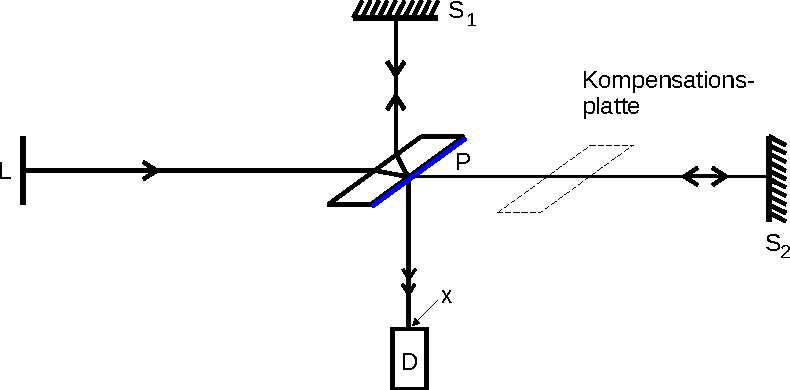
\includegraphics[width=0.75\textwidth]{figures/Abb1.pdf}
    \caption{Aufbau eines Michelson-Interferometers. In der Abbildung ist L die Lichtquelle, $\textrm{S}_1$ und $\textrm{S}_2$  Spiegel, P eine semipermeable Platte und D eine Photodiode \cite{ap11}.}
    \label{fig:Michelson}
\end{figure}

Das Licht aus dem Laser fällt auf eine semipermeable Platte. Ein Teil des Licht geht ohne Richtungsänderung durch diese hindurch. Der andere Teil wird senkrecht zur Einfallsrichtung reflektiert. 
Beide Teilstrahlen fallen  senkrecht auf die Spiegel $ \textrm{S}_1 $ und $ \textrm{S}_2 $, von denen sie reflektiert werden.
Die zurücklaufenden Strahlen fallen am Punkt P wieder zusammen und werden erneut gebrochen. 
Um kohärentes Licht zu erhalten, muss der Wegunterschied zwischen $\overline{S_1 P}$ und $\overline{S_2 P} $ kleiner sein als die Kohärenzlänge des Lasers.
Dazu ist es notwendig, eine Kompensationsplatte zwischen der semipermeablen Platte und $S_2$ einzufügen, da der Strahl von $S_2$ die semipermeable Platte nur einmal durchläuft und nicht dreimal wie der Strahl, der von $S_1$ reflektiert wird. 
Die Kompensationsplatte muss den gleichen Brechungsindex haben wie die semipermeable Platte.
Sollten die Abstände $\overline{S_1 P}$ und $\overline{S_2 P} $ genau gleich sein, interferiert das Licht am Detektor destruktiv, weil es eine $\lambda /2 $-Phasensprung des von $S_2$ kommenden Strahles gibt. \\

Wird einer der Spiegel um ein Stück $d$ verschoben, dann erhält der Strahl einen Gangunterschied von $w = 2d$ und die am Detektor gemessene Intensität ändert sich.
Wird der Abstand d kontinuierlich vergrößert oder verkleinert, variiert die Intensität am Detektor, mit der räumlichen Periode $\lambda / 2$. 
Wird der Spiegel um ein Stückchen $ \symup{\Delta} d$ verschoben, können die vorbeiziehenden Intensitätsminima gezählt werden.
Aufgrund dieser Periodizität kann der Aufbau zur Bestimmung der Wellenlänge des Lasers benutzt werden. 
Aus dieser Betrachtung kann \eqref{eq:deltad} motiviert werden.

%%%%%% Label mal die Formel, nach der wir Lambda berechnen (also Δd = z λ/2) mal bitte 'eq:deltad', dann passt das in der Auswertung alles schön :)
\begin{equation}
    \Delta d = z \lambda/2. 
    \label{eq:deltad}
\end{equation}

Ein Gangunterschied zwischen den beiden Lichtsprachen kann auch erzeugt werden, indem ein Lichtstrahl für ein Stück b ein optisch dichteres Medium durchläuft.
Ein solcher Aufbau ist in \autoref{fig:Abb2} dargestellt.
\begin{figure}[H]
    \centering
    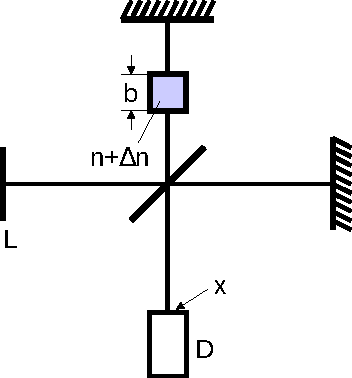
\includegraphics{figures/Abb2.pdf}
    \caption{Aufbau eines Michelson-Interferometers zur Bestimmung von Brechungsindizes durch Variation von Dichten \cite{ap11}.}
    \label{fig:Abb2}
\end{figure}

Für die Länge b durchläuft ein Lichtstrahl ein Medium mit dem Brechungsindex $ \Delta n + n$. Die optische Weglänge wird um ein $\Delta n b$ vergrößert.
Die Änderung des Brechungsindex kann durch eine Erhöhung des Gasdrucks, oder durch das Einschieben mehrerer optischer Platten geschehen.
Während der Brechungsindex geändert wird, laufen am Ort $x$ die Intensitätsminima vorbei. Diese können durch den Detektor gemessen werden.
Für eine Änderung des Brechungsindex um $\Delta n$ gilt die \eqref{eq:bdeltan}
%%%%%% Label mal die Formel b Δn = zλ/2 bitte 'eq:bdeltan'
\begin{equation}
    b \Delta n = z λ/2. 
    \label{eq:bdeltan}
\end{equation}
Damit aus $\Delta n$ der eigentliche Brechungsindex des Mediums bestimmt werden kann, muss \eqref{eq:brechungsindex} benutzt werden.
%%%%%% und die Formel n(p_0,T_0) = 1 + Δn T/T_0 p0/(p-p') bitte 'eq:brechungsindex' dange :D
\begin{equation}
    n(p_0,T_0) = 1 + \Delta n \frac{T}{T_0} \frac{p_0}{\rho - \rho'} .
    \label{eq:brechungsindex}
\end{equation}
